\documentclass[12pt,a4paper]{article}
\usepackage{enumerate} %put in numbers or bullet points
\usepackage{setspace}
\raggedright %justify the text on the left only
\usepackage{graphicx} 	% For adding pictures
\usepackage{float}
\usepackage{pdflscape}	% for landscape pages
\pagenumbering{arabic}	% Page numbers
\usepackage{fancyhdr} % add headers and footers
\usepackage{hyperref} % hyper links for references

\onehalfspacing %1.5 line spacing
\usepackage[round]{natbib} % author-year citations in round brackets


\begin{document}

\title{Convergence and disparity in the evolution of tenrecs}
\author{}
\date{}
\maketitle


%Add a header 
\renewcommand{\headrulewidth}{0.0pt}
\thispagestyle{fancy}				%header on the first page only
\lhead{Sive Finlay, Progress Report}
\chead{}
\rhead{May 2014}


\section{Introduction}
My PhD is an investigation of evolutionary patterns in tenrecs (Afrosoricida, Tenrecidae). My aim is to quantify both morphological and ecological diversity within the tenrec family (disparity) and their similarities to other small insectivorous mammals (convergence). 
I am now half way through my three year PhD and I have a plan of how my thesis will take shape. I included a provisional thesis outline of five chapters in my first year report in November 2013 (see attached document). However, based on the committee's advice that some of the chapters were too large and the fact that my fieldwork experiments did not go according to plan (see section three below), I have now modified my thesis.  The new plan is to have seven chapters, at least four of which will be paper-driven. I have included a draft outline of my first paper, "Cranial morphological disparity within the adaptive radiation of tenrecs (Afrosoricida, Tenrecidae) is no greater than expected by chance" which will comprise my third chapter.
In this report I outline my current progress and plans for completion of my papers and each chapter. I include the target date for completion of each paper/ chapter and summarise these targets in a GANNT chart timetable at the end of the report (figure \ref{gannt}). 

\newpage

\section{Thesis outline}

\begin{enumerate}
\item \textbf{Chapter 1: Introduction}\\
\textit{To be completed by November 2015 (figure \ref{gannt})}\\

This is a general introductory chapter. I will include brief outlines of convergence and disparity and why they are useful and interesting measures of evolutionary diversity. I will discuss convergence within the context of what it tells us about the repeatability of evolution \citep[e.g][]{Blount2008} and disparity within the framework of how it relates to the study of adaptive radiations \citep{Losos2010a}. In particular, I will stress the importance of taking quantiative approaches to studying each of these patterns rather than relying on subjective estimates. I will follow these discussions with a brief introduction of tenrecs and the long-standing interest in the apparently high morphological and ecological diversity within the family and the similarities among tenrecs and other distantly related mammal species \citep[e.g.][]{Eisenberg1969, Soarimalala2011, Olson2013}. 

Along with the conclusions (chapter seven), this will be the last chapter that I write because it will be easier to introduce the rest of the thesis once I know how those chapters have taken shape. 

\item \textbf{Chapter 2: Data collection}\\
\textit{To be completed by September 2014 (figure \ref{gannt})}\\
My thesis will be based on two main data sources; morphological and ecological. The questions addressed in chapters three, five and six will all be base on these same data sources. Therefore, rather than repeating the information in multiple sections, I will combine my data collection methods into this single chapter which I can then refer to in the rest of the thesis. 
I have collected all of the data and completed most of the writing for the morphological section of this chapter. I haven't started the sections relating to the ecological data but I will work on this aspect as I collect the relevant data over the coming months (see chapter six below). I will finish writing the chapter by this September.

\item \textbf{Chapter 3: Quantifying morphological disparity in tenrecs}\\
\textit{Journal targets: Journal of Evolutionary Biology, PLoS ONE, Journal of Mammalian Evolution? , submit August 2014. 
Complete chapter by June 2015 (figure \ref{gannt}}\\

This is the chapter which corresponds to the draft paper that accompanies this report. I have completed the majority of the work for this paper. Given that tenrecs are often cited as an example of a phenotypically diverse group \citep[e.g.][]{Olson2013}, my finding that morphological disparity is no greater than expected by chance was unexpected. Therefore I'm currently checking the code that I used for the calculations and simulation studies to ensure that the results are accurate rather than just artefacts of a fault in the methods. 

I would very much welcome any comments on the draft paper, particularly if you have suggestions for how I could make the overall story clearer and more interesting to a wide audience. My aim for the paper is that it's a test of a broad principle; the importance of testing our assumptions about phenotypic variation in adaptively radiated groups, with tenrecs as a specific example rather than a more limited study of morphological variation in a particular group of mammals.

Dr. Steve Goodman, an expert in tenrec ecology and evolution, has expressed an interest in collaborating on the paper so I will send it to him for comments before submitting to the Journal of Evolutionary Biology by the end of the summer.

\item \textbf{Chapter 4: Review of methods of detecting convergence}\\
\textit{Journal target: Journal of Evolutionary Biology, submit June 2015. Complete chapter by September 2015 (figure  \ref{gannt} )}

Convergence is a common evolutionary pattern of historical significance and interest because it relates to questions about the relative roles of determinism and contingency in evolution \citep[c.f][]{Blount2008}. Many studies of convergence are purely qualitative descriptions of apparent patterns of similarity among species \citep[e.g.][]{Ben-Moshe2001, Leal2002, Fleischer2008} including recent studies of genomic convergence \citep{Jones2012, Parker2013}. 

However, there is increasing interest in developing new metrics of quantifying the degree of convergent evolution among species. These quantitative approaches for assessing the significance of apparent convergence are particularly important in the wake of research which revealed that some level of convergence is expected to evolve by chance in most phylogenies \citep{Stayton2008}.
The discrepancies among these metrics have produced a confusing variety of techniques of quantifying convergence with no clear guidelines for the relative suitabilities of different methods or how they compare to each other.
   

This chapter will be a review of exising methods for quantifying convergence. It will serve as both a lead in for my subsequent chapter on quantifying convergence in tenrecs and it will also be a separate paper. 
I will start with a brief review of why convergence is important and interesting to study and the developing need for rigorous quantitative approaches. I will classify convergence studies into three primary groups; papers which are purely qualitative/descriptive (see examples above), papers which quantify convergence and papers which fall between the two extremes - they don't just look at patterns of convergence but they don't measure significance either  \citep[e.g.][]{Tseng2013, Kawahara2013, Wroe2007, Jones2007, Clark2005}. I will group the papers that do quantify convergence into methods for measuring convergence across a tree \citep{Stayton2008}, between species pairs \citep{Muschick2012, Stayton2006, Harmon2005} or lineages of species \citep{Revell2007} and methods for quantifying community/faunal convergence \citep{Burd2014, Alvarado2013, Ingram2013, Mahler2013, Moen2013, Segar2013, Elias2008, Melville2006}.  

While many of these metrics are seemingly sound and useful, they are usually developed using simulation studies and then only tested on relatively few biological groups, for which detailed morphological, ecological and phylogenetic data are well known. 
The realistic potential for application of each method to other data sets and questions is often more restricted than the authors suggest. Therefore I will summarise the approach of each method,comment on any potential problems and outline their suitability for other data sets and questions. This review will be useful for the rest of my own research but it will make a topical and interesting paper.  

There are many existing papers which review conceptual insights and investigations of convergent evolution \citep[e.g.][]{Losos2011, Conway-Morris2006, Scheffer2006} but my paper will be the first review of methods of measuring convergence. 

I have an outline plan of the chapter and I have already completed an initial literature review. I will add to this research when I'm using some of these methods to quantify convergence in my own data (see chapter five) and I will write the paper after I have completed my own analyses because that will give me a better understanding of the methods.


\item \textbf{Chapter 5: Quantifying morphological convergence among tenrecs and other small mammals}\\
\textit{Journal targets; Journal of Evolutionary Biology, PLoS ONE, submit January 2015. Complete chapter by August 2015 (figure \ref{gannt})}

Following on from my review of methods of quantifying convergence (chapter four) I will apply some of these methods to my data to measure the degree of morphological similarity among tenrecs and other distantly related small mammals (shrews, moles, hedgehogs, solenodons).
As I described previously in my November 2013 report, I have an extensive morphological data base of tenrecs and the mammals they resemble. I have completed my geometric morphometric analyses of all of the skull and mandible specimens and I can now move onto quantifying convergence.

%*******************************************
%Put in which methods I'm going to use - both for overall convergence of the family and between specific groups.
%***********************************

I will write these analyses into a paper about the general importance of quantifying convergence focusing on the specific example of tenrecs. Despite numerous claims and indications that tenrecs are convergent with other animal groups \citep[e.g.][]{Olson2013, Eisenberg1969, Soarimalala2011} this paper will be the first to test the hypothesis in a quantitative framework.

I think that my cranial analyses will be sufficient data for the paper. However, I also have a dataset of limb measurements which a final-year undergraduate is going to analyse for evidence of convergence this year. The results of her project will indicate whether it would be productive for me to include a straightforward analysis of my limb measurements (for example correlations between limb proportions and locomotion style/habitat) in my assessment of convergence.


\item \textbf{Chapter 6: Is morphological convergence between tenrecs and other mammals predicted by ecological similarity?}\\
\textit{Possible journals: Journal of Evolutionary Biology,PLoS ONE, submit April 2015. Complete chapter by September 2015 (figure \ref{gannt}) } 

Tenrecs are often cited as an example of an adaptive radiation in which species evolved to fill ecological niches which were vacant due to the absence of other small mammal competitors \citep[e.g.][]{Eisenberg1969}. It is assumed that this occupation of similar ecological niches led to the striking examples of phenotypic convergence among tenrecs and other small mammal species.  
However,given that ecological similarities are neither necessary nor sufficient for phenotypic convergence to evolve \citep{Losos2011}, it is important to test potential correlations between morphological and ecological similarities explicitly.

Building on my analyses of morphological convergence (chapter 5), here I will quantify the relationship between phenotypic and ecological similarities among my species.
I outlined my plans for ecological data collection in my November 2013 report (attached). I originally intended to collect the data in the spring of this year but my disparity analyses and preparations for fieldwork (see section three) took precedence. Therefore I plan to collect the relevant data (using the sources outlined in section 3.2 of the  November 2013 report) over the summer. The end of this data collection period will overlap with my analyses of morphological convergence which will give me time to clean-up the ecological data and hone my skills at quantifying convergence in general before I come to analysing the ecological data (see figure \ref{gannt}). 

I will approach data analysis in two stages. The first will be a straightforward (and, I think, appropriate) assessment of niche similarities derived from a pairwise distance matrix from a principal components analysis of all niche variables \citep[e.g.][]{Melville2006}. This will give me a measure of pairwise niche (dis)similarity among all species which I can then compare to my morphological distance matrices. Here the prediction is that morphologically convergent species pairs will be separated by smaller ecological distances. The new Wheatsheaf index method of quantifying the degree of convergence \citep{Arbuckle2014} could be appropriate here as it's a phylogenetically-weighted measure of similarity among convergent groups which have been identified \textit{a priori}. I can also modify the methods in \citep{Muschick2012} to compare morphological and ecological distances.

The second option is to build species distribution models and to quantify ecological convergence as niche overlap \citep{Rodder2011}.


\item \textbf{Chapter 7: Conclusions}\\
\textit{Complete chapter by November 2015 (figure \ref{gannt})}

This chapter will summarise the importance of taking a quantitative approach to studies of evolutionary diversity (morphological and ecological) among species groups. In particular I will highlight the need to apply existing methods to new groups of species which are usually not as well studied as the groups that are used to develop such metrics. I will also include suggestions for future directions, particularly in the area of addressing the functional importance rather than pure description of convergent traits \citep{Losos2010}. I could also include mention my unsuccessful fieldwork experiments here (see below) as another potential basis for future work. 

\end{enumerate}

\section{Unsuccessful fieldwork for testing behavioural convergence}

In my November 2013 report I outlined my plans for incorporating tests of behavioural convergence into my project. I was interested in whether early reports of an ability to echolocate in some tenrecs \citep{Gould1965} may be extended to other species of the \textit{Microgale} (shrew-type) tenrecs and therefore provide evidence of behavioural convergence between tenrecs and shrews \citep{Siemers2009}. Natalie and I went to Madagascar in March/April as part of a research trip led by Dr.Steve Goodman to conduct behavioural tests of echolocation in \textit{Microgale}. Our aim was to record the sounds made by the animals as they moved through a wooden maze towards a food reward to determine whether there was evidence that they were using sounds to navigate through their environment. We tried multiple variations of our protocol but unfortunately none of the animals we tested produced any noise (17 individuals from 5 different species). It is clear that this negative result is a failure of our experiment rather than an indication that \textit{Microgale} don't navigate using sounds. Our sample included \textit{Microgale dobsoni} which are one of the few species which are known to echolocate from previous experiments \citep{Gould1965}. Similarly, other more experienced researchers in the group had heard the \textit{Microgale} making sounds while foraging. Previous studies of echolocation in small mammals \citep{Gould1964, Gould1965, Tomasi1979, Siemers2009} all used captive individuals which were trained to perform specific tasks. Such a prolonged procedure was not possible wihtin our constraints of time and facilities.

Given that I have no useable data to address my questions of behavioural convergence it is not enough information for a complete chapter. I could mention the experiments briefly in my concluding chapter as an idea for further directions. Alternatively, I could leave these investigations of behavioural convergence out of the thesis altogether to avoid detracting from my more general studies of morphological and ecological (dis)similarities among species.

\section{Other work}
\begin{enumerate}

\item \textbf{Publications since the November 2013 report}\\
\textbf{Finlay, S.}, Goodman, S.M., Cooper, N. Significant levels of morphological disparity in the adaptive radiation of tenrecs (Afrosoricida, Tenrecidae). \textit{In prep. To be submitted to the Journal of Evolutionary Biology}\\
\bigskip %skip a line between the two references
Healy, K., Guillerme T., \textbf{Finlay, S.,}, Kane, A., Kelly, S.B.A., McClean, D., Kelly, D.J., Donohue, I., Jackson, A.L. and Cooper, N., 2014.Ecology and mode-of-life explain lifespan variation in birds and mammals. \textit{Proceedings of the Royal Society B, 281(1784)} 

\item \textbf{Presentations}\\
This summer I will give my first oral conference presenations at the Evolution conference in Raleigh, North Carolina (June) and the British Ecological Society Macroecology conference in Nottingham (July).

\item \textbf{Reviewing}\\

So far I have reviewed a journal article (International Journal of Primatology) and a book chapter on phylogenetic comparative methods for quantifying convergence. I hope that I will get some more reviewing practice once I start publishing my own papers.



\end{enumerate}


\begin{landscape}
\begin{figure}[p]
\centering
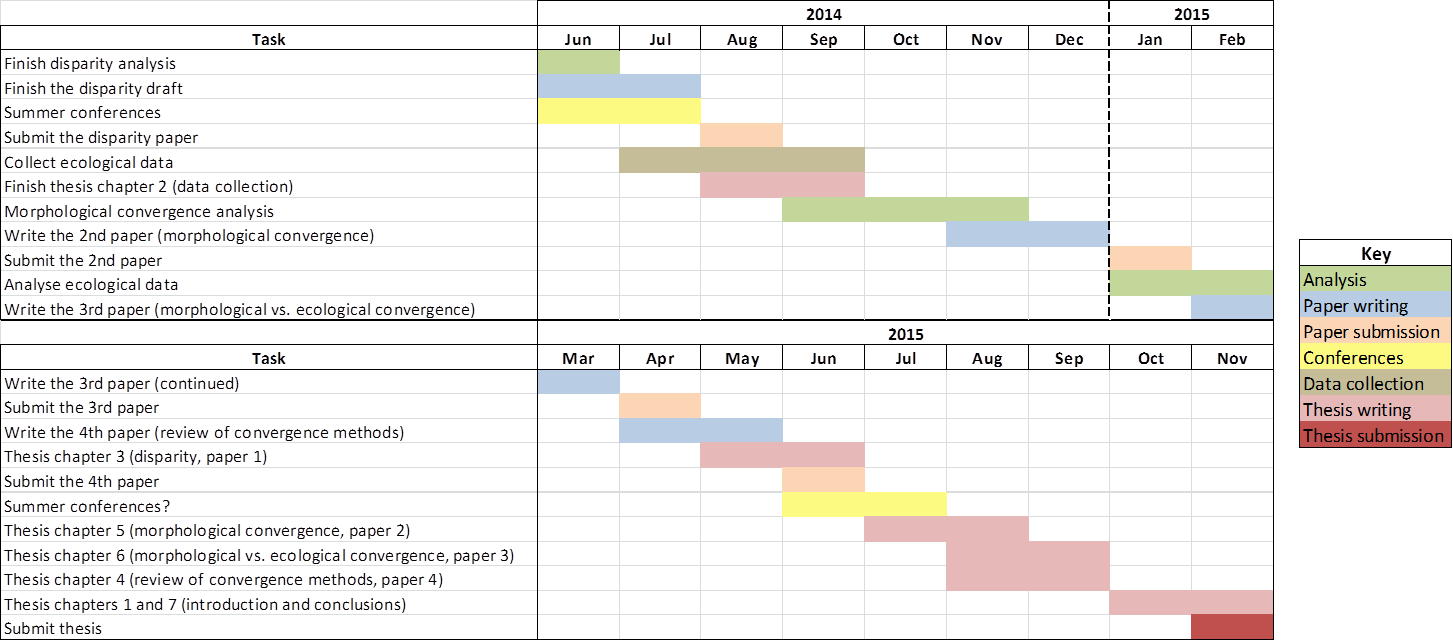
\includegraphics[keepaspectratio=true]{Gannt+key.png}
\caption{Timeline for completion of my PhD, tasks are colour coded following the accompanying key}
\label{gannt}
\end{figure}
\end{landscape}



\bibliographystyle{jeb}
\bibliography{Refs_01_05_14_edited} %This is my edited JabRef file of all my references exported from EndNote. I had to edit the formatting for the special characters, capital letters and also change the file encoding.


\end{document}